Given the following regression model:
$$
RPmsoft_t = \beta_1 + \beta_2RPsandp_t + \beta_3 Dprod_t + \beta_4Dinflation_t + \beta_5Dterm_t + \beta_6m1_t + \epsilon_t
$$

where 
\begin{itemize}[label=(alpha*)]
    \item[-] $RPmsoft_t$ is the excess return of the Microsoft stock,
    \item[-] $RPsandp_t$ is the risk premium of the S\&P 500 index,
    \item[-] $Dprod_t$ is the change in production,
    \item[-] $Dinflation_t$ is the change in inflation,
    \item[-] $Dterm_t$ is the change in term structure,
    \item[-] $m1_t$ is the money supply growth,
    \item[-] $\epsilon_t$ is the error term.
\end{itemize}

\subsection{}
Using the data microsoft.csv, the resulting regression model is as follows:

\begin{align*}
\widehat{RPmsoft_t} = -0.9291 + 1.3232RPsandp_t -1.5216Dprod_t \\  + 0.4716Dinflation_t + 4.1588Dterm_t + 5.4352m1_t 
\end{align*}

\begin{center}
\fbox{
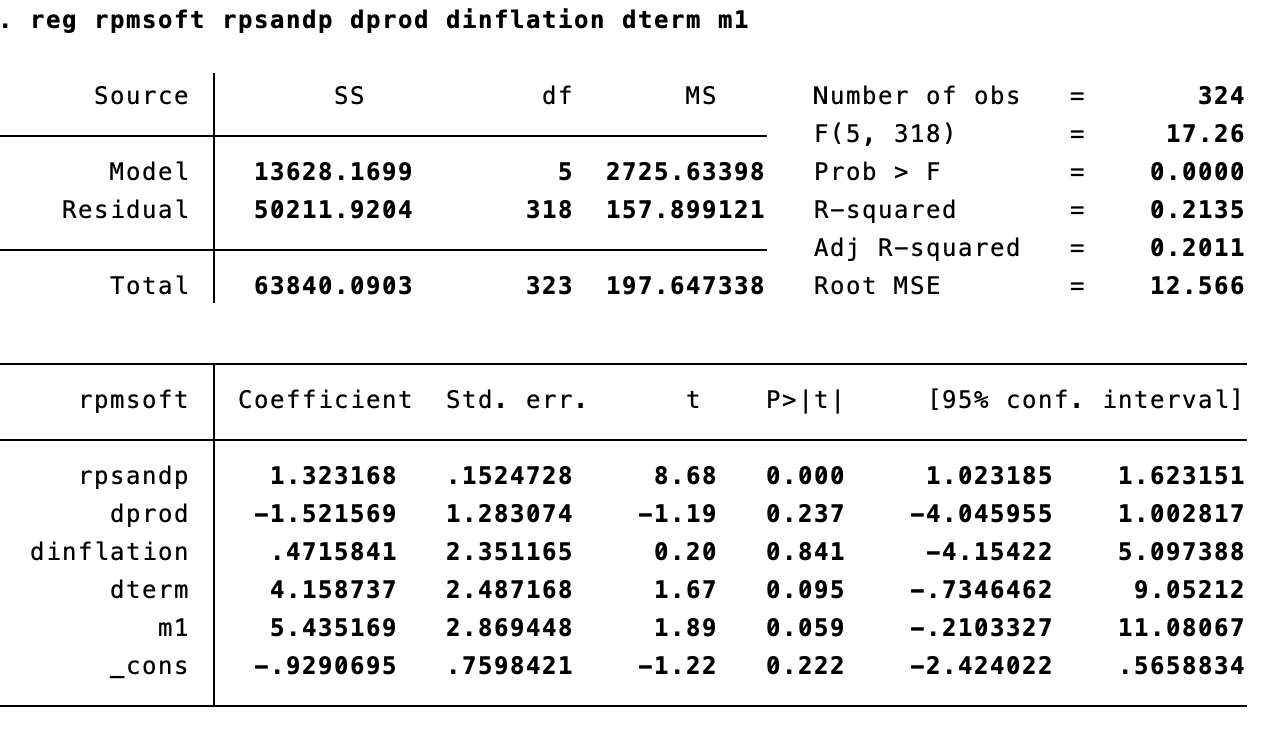
\includegraphics[width=12cm]{fig/2a.png}
}
\end{center}

\subsection{}
To test the \textit{January effect} which is that on avereage, every else equal, the returns (or excess returns) are larger in the month of January than the rest of the months, we set-up the following hypothesis test:

$$
H_0: \beta_6 = 0 \quad \text{(No January effect)} \quad vs \quad
H_a: \beta_6 > 0 \quad \text{(January effect exists and is positive)}
$$

where $\beta_6$ is the estimated coefficient for the regressor $m1$ which is a 1 for January and 0 otherwise. 

\medskip 

From there OLS regression results, we have $t-value = 1.89$. At $\alpha=1\%$ and degrees of freedom  $n-K = 324 - 6 = 298$, the $t-critical_{0.01}(298) = 2.339$. Because $t-value < t-critical$, we fail to reject the null hypothesis. That is, the data does not provide evidence to reject the claim that there is no January effect in the excess returns of Microsoft stock.

\subsection{}

The starting point for use of the $t-test$ statistic is the (conditional) sampling distribution of the $\hat{\beta}_k$ which is derived from the classifical assumptions plus normality. Thus, the assumptions other than normality are:

\begin{enumerate}[label=(A\arabic*)]
    \item Linearity: The regression model has been correctly specified such that $y = X\beta + \epsilon$ 
    \item Strict exogeneity: The error term has an expected value of zero given any values of the regressors in all time periods, i.e. $E(\epsilon_i | X) = 0$ for all $i$.
    \item Homoskedasticity: The variance of the error term is constant across all levels of the regressors, i.e. $Var(\epsilon_i | X) = \sigma^2$ for all $i$.
    \item Disturbances are uncorrelated: The error terms are uncorrelated across observations,
    i.e. \\ $Cov(\epsilon_i, \epsilon_j | X) = 0$ for all $i \neq j$.
\end{enumerate} 

In addition, to derive the distribution of the $t-test$ statistic, we used 

$$\dfrac{\hat{\beta_k} - r}{\sqrt{\sigma^2(X'X)^{-1}_{kk}}} \quad \underset{\text{under }H_0}{\sim} \quad  N(0,1)$$

where $r$ is the value of $\beta_k$ under the null hypothesis. Thus, the distribution of the $t-test$ statistic is derived under the assumption that $H_0$ is true.

\subsection{}

The $Jarque-Bera$ (JB) test can be used to check for normality of the distrubances. The JB-test statistic is given by:
$$JB = \dfrac{n}{6} \left( sk^2 + \dfrac{(kur-3)^2}{4} \right) \quad \overset{a}{\underset{\text{under }H_0}{\sim}} \quad \chi^2(2)$$
where $sk$ is the sample coefficient of the skewness of the variable, $kur$ is its sample coefficient of kurtosis, and $n$ is the sample size. Using significance of level of $\alpha = 0.01$ and the critical value $X^2_{0.01}(2) = 9.21$. The acceptance and rejection regions are in the illustration below:

\begin{center}
\fbox{
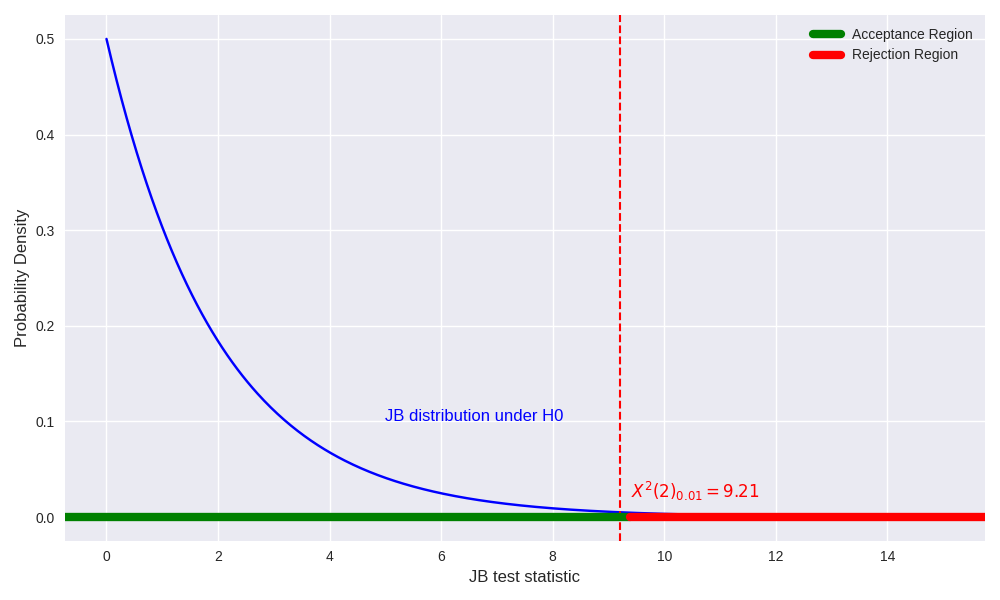
\includegraphics[width=12cm]{fig/2d.png}
}
\end{center}

A normal distribution has skewness of 0 and kurtosis of 3.  Thus, a deviation from these values can indicate a departure from normality. The corresponding hypothesis test is set-up as follows:
$$
H_0: SK = 0 \text{ and } KUR = 3  \quad vs \quad H_A: \text{ not } H_0
$$

where $SK$ and $KUR$ are the population coefficients of skewness and kurtosis for the disturbances, respectively. 

Under normality, the mean and variance of skewness is 0 and $\frac{6}{n}$ and 3 and $\frac{24}{n}$ for kurtosis, respectively. Thus, we can see the $JB-test$ statistic is composed of mahalonobis distances for $SK$ and $KUR$. If the disturbances are normally distributed, then the $JB-test$ statistic should be small, otherwise it will have a large positive value. Therefore, the acceptance region is from 0 up to the critical value determined by the significance level.
\subsection{}
If the assumptions regarding the $dgp$  for conistency of $OLS$ estimator are met, then $\hat{\beta} \overset{p}{\rightarrow} \beta$. Note that $\hat{\epsilon} = y - \hat{y} =  X\beta + \epsilon - X\hat{\beta} = X(\beta - \hat{\beta}) + \epsilon$, by \textit{Continuous Mapping Theorem}, we have  $\hat{\epsilon} \overset{d}{\rightarrow} X(\beta - \beta) + \epsilon = \epsilon$. Thus, $\hat{\epsilon} \overset{d}{\rightarrow} \epsilon$.

\subsection{}

Using Stata, the $JB-test$ value is 1809. At $\alpha=0.01$ and degrees of freedom  = 2, the critical value is $X^2_{0.01}(2) = 9.21$. Since 1809>9.21, we reject the null hypothesis that the disturbances are normally distributed. Thus, there is evidence to suggest that the disturbances are not normally distributed.

\subsection{}
Testing again the $January$ $effect$ using asymptotic t-test, we have critical value =  $z_{0.01}$ = 2.326. Since the $t-value = 1.89 < 2.326$, we fail to reject the null hypothesis. Thus, the conclusion remains the same as in part (b) that there is no evidence to suggest the existence of January effect in the excess returns of Microsoft stock. 

\subsection{}
Yes. Because the normality assumption for the exact $t-test$ is not satisfied

\subsection{}
The $t-test$ statistic distribution has fatter tails than the standard normal distribution or the $z$ statistic. This means that at the tails, using the same significance level, the value of the $t-test$ statistic will be smaller that the $z$ statistic.